\documentclass[a4paper]{article}

\usepackage{fullpage} % Package to use full page
\usepackage{parskip} % Package to tweak paragraph skipping
\usepackage{tikz} % Package for drawing

\usepackage{hyperref}
\usepackage{amsmath}
\usepackage{amssymb}
\usepackage{amsthm}
\usepackage{enumitem}

\usepackage{subcaption}

\title{COMP 339 Assignment 3}
\author{Ling Tan}
\date{2018/11/05}

\begin{document}

\maketitle

\section{}
\begin{enumerate}[label=\alph*)]
      \item Let $G$ be an undirected graph with $n$ vertices. If $G$ is isomorphic to its own complement $\Bar{G}$, how many edges must $G$ have? (Such a graph is called \textit{self-complementary}).\\
          \textcolor{blue}{Answer:}\\
          Let $G=(V,E)$ and $\Bar{G}=(V,\Bar{E})$,\\
          $G$ is self-complementary $\Rightarrow|E|=|\Bar{E}|$ and $|E|+|\Bar{E}|=\binom{n}{2}$.\\
          That is, G must have $\frac{1}{2}\binom{n}{2}$ edges.
      \item Find an example of a self-complementary graph on four vertices and one on five vertices.\\
          \textcolor{blue}{Answer:}
          \begin{itemize}
              \item $4$ vertices:
                \begin{figure}[!htbp]
                    \begin{subfigure}[!htbp]{0.5\textwidth}
                        \centering
                        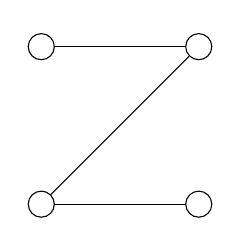
\begin{tikzpicture}[auto]
                            \begin{scope}[every node/.style={circle,draw=black,minimum size=3mm}]
                                \node (A) at (-1,0) {};
                                \node (B) at (1,0) {};
                                \node (C) at (-1,-2) {};
                                \node (D) at (1,-2) {};
                            \end{scope}
                            \begin{scope}[every edge/.style={draw=black}]
                                \draw (A) edge node{} (B);
                                \draw (B) edge node{} (C);
                                \draw (C) edge node{} (D);
                            \end{scope}
                        \end{tikzpicture}
                    \caption{$G_4$}
                    \end{subfigure}
                    \begin{subfigure}[!htbp]{0.32\textwidth}
                        \centering
                        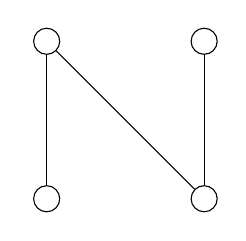
\begin{tikzpicture}[auto]
                            \begin{scope}[every node/.style={circle,draw=black,minimum size=3mm}]
                                \node (A) at (-1,0) {};
                                \node (B) at (1,0) {};
                                \node (C) at (-1,-2) {};
                                \node (D) at (1,-2) {};
                            \end{scope}
                            \begin{scope}[every edge/.style={draw=black}]
                                \draw (C) edge node{} (A);
                                \draw (A) edge node{} (D);
                                \draw (D) edge node{} (B);
                            \end{scope}
                        \end{tikzpicture}
                        \caption{$\Bar{G_4}$}
                    \end{subfigure}
                \end{figure}
              \item $5$ vertices:
                \begin{figure}[!htbp]
                    \begin{subfigure}[!htbp]{0.5\textwidth}
                        \centering
                        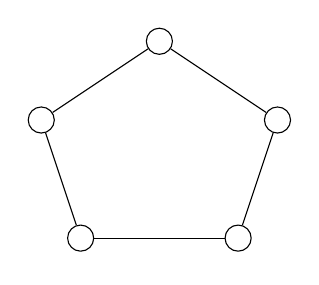
\begin{tikzpicture}[auto]
                            \begin{scope}[every node/.style={circle,draw=black,minimum size=3mm}]
                                \node (A) at (0,0) {};
                                \node (B) at (1.5,-1) {};
                                \node (C) at (1,-2.5) {};
                                \node (D) at (-1,-2.5) {};
                                \node (E) at (-1.5,-1) {};
                            \end{scope}
                            \begin{scope}[every edge/.style={draw=black}]
                                \draw (A) edge node{} (B);
                                \draw (B) edge node{} (C);
                                \draw (C) edge node{} (D);
                                \draw (D) edge node{} (E);
                                \draw (E) edge node{} (A);
                            \end{scope}
                        \end{tikzpicture}
                        \caption{$G_5$}
                    \end{subfigure}
                    \begin{subfigure}[!htbp]{0.32\textwidth}
                        \centering
                        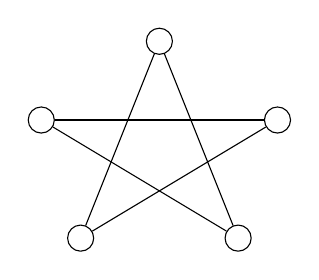
\begin{tikzpicture}[auto]
                            \begin{scope}[every node/.style={circle,draw=black,minimum size=3mm}]
                                \node (A) at (0,0) {};
                                \node (B) at (1.5,-1) {};
                                \node (C) at (1,-2.5) {};
                                \node (D) at (-1,-2.5) {};
                                \node (E) at (-1.5,-1) {};
                            \end{scope}
                            \begin{scope}[every edge/.style={draw=black}]
                                \draw (A) edge node{} (C);
                                \draw (A) edge node{} (D);
                                \draw (B) edge node{} (D);
                                \draw (B) edge node{} (E);
                                \draw (E) edge node{} (C);
                            \end{scope}
                        \end{tikzpicture}
                        \caption{$\Bar{G_5}$}
                    \end{subfigure}
                \end{figure}
          \end{itemize}
      \item If $G$ is self-complementary graph on $n$ vertices, where $n>1$, prove that $n=4k$ or $n=4k+1$, for some $k\in\mathbb{Z^+}$.\\
        \textcolor{blue}{Answer:}
        \begin{proof}
            Let $G=(V,E)$ and $\Bar{G}=(V,\Bar{E})$. $G$ is self-complementary $\Rightarrow|E|=|\Bar{E}|$ and $|E|+|\Bar{E}|=\binom{n}{2}$.\\
            That is, $|E|=\frac{1}{2}\binom{n}{2}=\frac{(n)(n-1)}{4}$\\
            $\Rightarrow (n)(n-1)=4|E|$\\
            $\Rightarrow n=4k$ or $n-1=4k\Rightarrow n=4k$ or $n=4k=1, k\in\mathbb{Z^+}$.
        \end{proof}
    \end{enumerate}

\section{}
\begin{enumerate}[label=\alph*)]
    \item Find the number of edges in $Q_8$.\\
        \textcolor{blue}{Answer:} $2^{10}$.
    \item Find the maximum distance between pairs of vertices in $Q_8$. Given an example of one such pair that achieves this distance.\\
        \textcolor{blue}{Answer:} The maximum distance is $8$. It's too difficult to draw it (clearly), but if we use $\mathbb{R}^8$ to represent the space of $Q_8$, then one example is from the point $(0,0,0,0,0,0,0,0)$ to the point $(1,1,1,1,1,1,1,1)$.
    \item Find the length of a longest path in $Q_8$.\\
        \textcolor{blue}{Answer:} The length of a longest path is $2^8-1$.
\end{enumerate}

\section{}
For $n\in\mathbb{Z^+}$, how many distinct (though isomorphic) paths of length $2$ are there in the $n$-dimensional hypercute $Q_n$?\\
    \textcolor{blue}{Answer:} $\binom{n}{2}\cdot2^n$.

\section{}
Prove that for each $n\in\mathbb{Z^+}$ there exists a loop-free connected undirected graph $G=(V,E)$, where $|V|=2n$ and which has two vertices of degree $i$ for every $1\leq i\leq n$.\\
    \textcolor{blue}{Answer:}
    \begin{proof} By induction.
        \begin{enumerate}
            \item Base: $n=1\Rightarrow |V|=2, |E|=1, deg(A)=deg(B)=1$.\\
                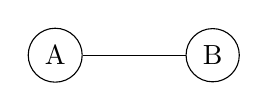
\begin{tikzpicture}[auto]
                    \begin{scope}[every node/.style={circle,draw=black,minimum size=3mm}]
                        \node (A) at (-1,0) {A};
                        \node (B) at (1,0) {B};
                    \end{scope}
                    \begin{scope}[every edge/.style={draw=black}]
                        \draw (A) edge node{} (B);
                    \end{scope}
                \end{tikzpicture}
            \item IH: Assume the statement is true for $1\leq k\leq n-1$.
            \item IS: Must prove the statement is true for $n$.
            \item Proof: By IH, we know that there exists a graph $G=(V,E), |V|=2(n-1)$ that has two vertices of degree $i$ for every $1\leq i\leq (n-1)$. Assume for $G, deg(v_i)=deg(v_i')=i$, for $1\leq i\leq n-1$.
                \begin{enumerate}
                    \item Add two vertices $v_n, v_n'$ to $G$, we formed a new graph $G'$ with $|V'|=2n$.
                    \item Connect $v_n$ and $v_n'$, we have $deg(v_n)=deg(v_n')=1$.
                    \item Connect $v_n$ to $v_1,v_2,\ldots, v_{n-1}$ respectively; connect $v_n'$ to $v_1',v_2',\ldots, v_{n-1}'$ respectively. We have $deg(v_n)=deg(v_n')=1+(n-1)=n, deg(v_i)=deg(v_i')=i+1$, for $1\leq i\leq n-1$.
                    \item Disconnect $v_{2i+1}$ and $v_{2i+2}$; disconnect $v_{2i+1}'$ and $v_{2i+2}'$ for $0\leq i\leq (n-3)/2\Rightarrow deg(v_i)=deg(v_i')=i$, for $1\leq i\leq n-1$.
                    \item That is, $G'$ has two vertices of degree $i$ for every $1\leq i\leq n$.
                \end{enumerate}
        \end{enumerate}
    \end{proof}

\section{}
Let $k$ be a fixed positive integer and let $G=(V,E)$ be a loop-free undirected graph, where $deg(v)\geq k$ for all $v\in V$. Prove that $G$ contains a path of length $k$.\\
    \textcolor{blue}{Answer:}
    \begin{proof} By contradiction.\\
    Assume $P_m=\langle v_1,v_2,\ldots, v_m\rangle$ is a path with maximum length $m-1$ in $G\Rightarrow$ there is no edge between $v_m$ and any vertex in $V\backslash \{v_1,v_2,\ldots, v_m\}$.\\
    Because if there is an edge, say $\{v_m, v_x\}$, then $\langle v_1,v_2,\ldots, v_m, v_x\rangle$ is a path with a longer length $m$, which contradicts to the assumption. That is, $v_m$ can only be adjacent to $v_1,v_2,\ldots,v_{m-1}\Rightarrow deg(v_m)\leq m-1$.\\
    Because $deg(v_m)\geq k$ is given $\Rightarrow k\leq m-1=length(P_m)$.\\
    That is, $G$ contains a path of length $k$.
    \end{proof}
    
\section{}
What is the length of a longest path in each of the following graphs?
\begin{enumerate}[label=\alph*)]
    \item $K_{1,4}$\hspace{2em}\textcolor{blue}{Answer:2}
    \item $K_{3,7}$\hspace{2em}\textcolor{blue}{Answer:6}
    \item $K_{7,12}$\hspace{2em}\textcolor{blue}{Answer:14}
    \item $K_{m,n}$, where $m,n\in\mathbb{Z^+}$ with $m<n$.\hspace{2em}\textcolor{blue}{Answer:$2m$}
\end{enumerate}

\section{}
\begin{enumerate}[label=\alph*)]
    \item Find all the nonisomorphic complete bipartite graphs $G=(V,E)$, where $|V|=6$.\\
        \textcolor{blue}{Answer:} $K_{1,5},K_{2,4},K_{3,3}$
    \item How many nonisomorphic complete bipartite graphs $G=(V,E)$ satisfy $|V|=n\geq2$?\\
        \textcolor{blue}{Answer:} $\lfloor n/2\rfloor$
\end{enumerate}

\section{}
\begin{enumerate}[label=\alph*)]
    \item Let $G=(V,E)$ be a loop-free connected graph with $|V|\geq11$. Prove that either $G$ or its complement $\Bar{G}$ must be nonplanar.\\
        \textcolor{blue}{Answer:}
        \begin{proof} By contradiction.\\
        Assume both $G=(V,E)$ and $\Bar{G}=(V,\Bar{E})$ are planar, $v=|V|=n, e_1=|E|,e_2=|\Bar{E}|$.
            \begin{align*}
                e&\leq3v-6\\
                e_1+e_2&\leq (3v-6)+(3v-6)\\
                |E|+|\Bar{E}|&\leq 6v-12\\
                \binom{n}{2}&\leq 6v-12=6n-12\\
                {(n)(n-1)}/{2}&\leq 6n-12\\
                n^2-13n+24&\leq 0
            \end{align*}
            Let $f(n)=n^2-13n+24,n\in\mathbb{Z^+}\Rightarrow f(n)\leq0$ for $2<n<11$.\\
            But $n=|V|\geq11$ is given, this contradicts to $2<n<11$, thus our assumption did not follow; so either $G$ or $\Bar{G}$ must be nonplanar.
        \end{proof}
    \item The result in part (a) is actually true for $|V|\geq 9$, but the proof for $|V|=9,10$ is much harder. Find a counterexample to part (a) for $|V|=8$.\\
        \textcolor{blue}{Answer:}
        \begin{figure}[!htbp]
            \begin{subfigure}[!htbp]{0.5\textwidth}
                \centering
                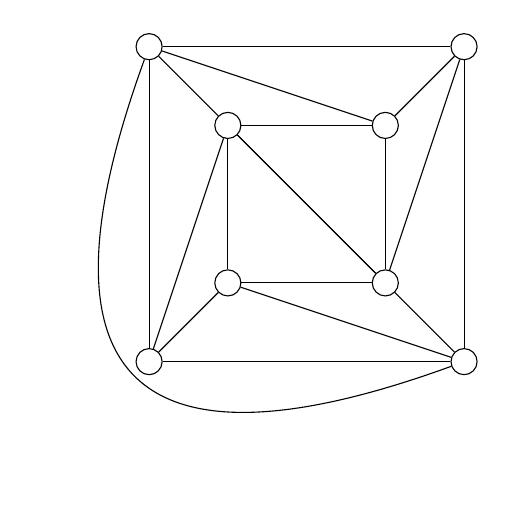
\begin{tikzpicture}[auto]
                    \begin{scope}[every node/.style={circle,draw=black,minimum size=3mm}]
                        \node (A) at (-2,2) {};
                        \node (B) at (2,2) {};
                        \node (C) at (2,-2) {};
                        \node (D) at (-2,-2) {};
                        \node (A1) at (-1,1) {};
                        \node (B1) at (1,1) {};
                        \node (C1) at (1,-1) {};
                        \node (D1) at (-1,-1) {};
                    \end{scope}
                    \begin{scope}[every edge/.style={draw=black}]
                        \draw (A) edge node{} (B);
                        \draw (B) edge node{} (C);
                        \draw (C) edge node{} (D);
                        \draw (D) edge node{} (A);
                        \draw (A1) edge node{} (B1);
                        \draw (B1) edge node{} (C1);
                        \draw (C1) edge node{} (D1);
                        \draw (D1) edge node{} (A1);
                        \draw (A) edge node{} (A1);
                        \draw (B) edge node{} (B1);
                        \draw (C) edge node{} (C1);
                        \draw (D) edge node{} (D1);
                        \draw (A1) edge node{} (C1);
                        \draw (A1) edge node{} (C1);
                        \draw (A) edge node{} (B1);
                        \draw (B) edge node{} (C1);
                        \draw (C) edge node{} (D1);
                        \draw (D) edge node{} (A1);
                        %\draw (A) edge [controls= +(250:5) and +(210:4)] node{} (C);
                        \draw (A) edge [out=250,in=200,looseness=2] (C);
                        %\draw plot [smooth,tension=1] coordinates { (-2,1.848) (-2.3,-2.3) (1.848,-2)};
                    \end{scope}
                \end{tikzpicture}
            \caption{$G_8$}
            \end{subfigure}
            \begin{subfigure}[!htbp]{0.32\textwidth}
                \centering
                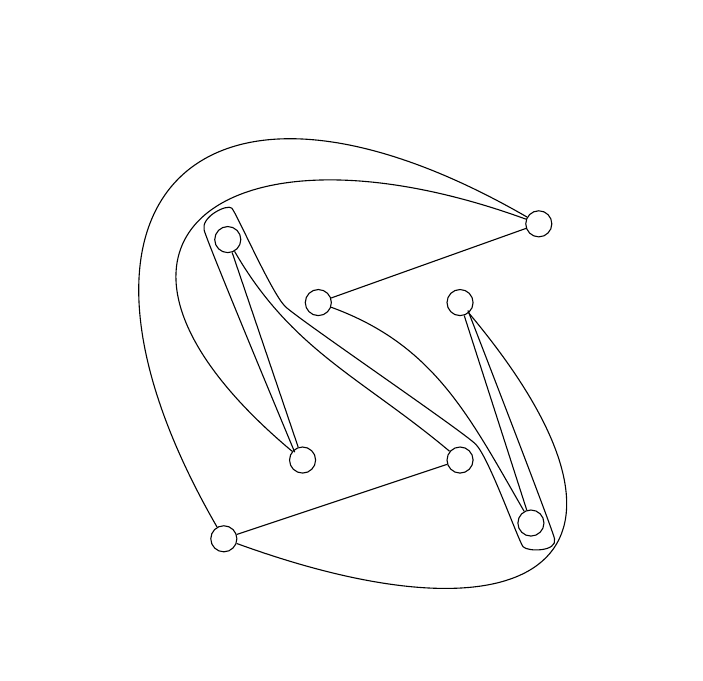
\begin{tikzpicture}[auto]
                    \begin{scope}[every node/.style={circle,draw=black,minimum size=3mm}]
                        \node (A) at (-1.95,1.8) {};
                        \node (B) at (2,2) {};
                        \node (C) at (1.9,-1.8) {};
                        \node (D) at (-2,-2) {};
                        \node (A1) at (-0.8,1) {};
                        \node (B1) at (1,1) {};
                        \node (C1) at (1,-1) {};
                        \node (D1) at (-1,-1) {};
                    \end{scope}
                    \begin{scope}[every edge/.style={draw=black}]
                        \draw (A) edge [out=300,in=140,looseness=1] (C1);
                        \draw (A) edge node{} (D1);
                        \draw (B) edge [out=150,in=120,looseness=2.2] (D);
                        \draw (B) edge node{} (A1);
                        \draw (B) edge [out=160,in=140,looseness=2.5] (D1);
                        \draw (C) edge [out=120,in=340,looseness=1] (A1);
                        \draw (C) edge (B1);
                        \draw (D) edge [out=340,in=310,looseness=2.5] (B1);
                        \draw (D) edge node{} (C1);
                        %\draw (B1) edge (D1);
                        \draw plot [smooth,tension=0.2] coordinates { (-1.1,-0.9) (-2.25,1.92) (-1.9,2.2)  (-1.22,0.95) (1.2,-0.8) (1.8,-2.1) (2.2,-2) (1.1,0.9)};
                    \end{scope}
                \end{tikzpicture}
                \caption{$\Bar{G_8}$}
            \end{subfigure}
        \end{figure}
\end{enumerate}
\section{}
Can a bipartite graph contain a cycle of odd length? Explain.\\
 \textcolor{blue}{Answer:} No. Because for a bipartite, if we start from either partition of the bipartite, to form a cycle we have to come back to that partition, so the length is always even.
\section{}
Let $G=(V,E)$ be a loop-free connected planar graph If $G$ is isomorphic to its dual and $|V|=n$, what is $|E|$?\\
\textcolor{blue}{Answer:} isomorphic $\Rightarrow |V|=r=n$. By $v-e+r=2\Rightarrow n-|E|+n=2\Rightarrow |E|=2n-2$.

\section{}
If $G = (V,E)$ is a connected graph with $|E| = 17$ and $deg(v) > 2$ for all vertices of graph $G$, what is the maximum value for $|V|$.\\
\textcolor{blue}{Answer:} $\sum_{v\in V}{deg(v)}=2|E|\Rightarrow 2|E|\geq 2|V|\Rightarrow |V|\leq |E|=17$.

\section{}
Prove that any subgraph of a bipartite graph is bipartite. \\
\textcolor{blue}{Answer:} 
\begin{proof} By contradiction.\\
Assume there is a subgraph $G'=(V',E')$ of a bipartite graph $G=(V,E)$ that is not bipartite.\\
That is, there is at least one pair of vertices in one of the two sets $P'$ and $Q'$ of $G'$ where $P'\cup Q'=V', P'\cap Q'=\emptyset$, say the edge $e'=\{x,y\}$ and $x,y\in P',e'\in E'$.\\
$G'\subseteq G, e'\in E'\Rightarrow e'\in E\Rightarrow G$ is not a bipartite $\Rightarrow$ Contradiction.
\end{proof}

\section{}
Let $G =(V,E)$ be an undirected connected loop-free planar graph. Suppose $G$ determines $53$ regions. If, for some planar embedding of $G$, each region has at least five edges in its boundary, prove that $|V| > 81$.\\
\textcolor{blue}{Answer:} 
Each boundary is counted twice $\Rightarrow 2|E|\geq 5r$.\\
By $v-e+r=2\Rightarrow |V|=2+|E|-r$.\\
$2|E|\geq 5r\Rightarrow |V|\geq 2+5/2r-r=2+3/2r=2+3/2\cdot 53\approx81.5>81$.


\section{}
\begin{enumerate}[label=\alph*)]
    \item  If graph $G$ is self-complementary (see Problem 1) 
        \begin{enumerate}[label=(\roman*)]
            \item determine $|E|$ if $|V| = n$;
            \item Prove that $G$ is connected.
        \end{enumerate}
    \item Let $n = 4k$ or $n = 4k + 1$ for non-negative number $k$. Prove that there exist a self-complementary graph $G = (V,E)$, where $|V| = n$.
\end{enumerate}
\textcolor{blue}{Answer:} 
\begin{enumerate}[label=\alph*)]
    \item Let $G=(V,E), \Bar{G}=(V',E')$.
        \begin{enumerate}[label=(\roman*)]
            \item $K_n=\binom{n}{2}\Rightarrow |E|=|E'|=1/2\binom{n}{2}$
            \item 
                \begin{proof} By contradiction.\\
                    Assume $G$ with two components $C_1,C_2$ is not connected.\\ For every pair of vertices in $V$, say $(x,y)$, if $x,y\in C_i, i=1,2$, they are connected in $G'$ through a vertex in other other component; if $x,y$ are in different components, then they are connected in $G'$ directedly. That is, $G'$ is connected.\\
                    But $G'$ is isomorphic to $G$, so $G$ has to be connected too, which leads to a contradiction.\\
                    So $G$ cannot be disconnected.
                \end{proof}
        \end{enumerate}
    \item
        \begin{proof} By induction on $k$.
            \begin{enumerate}
                \item Base: $k=1\Rightarrow n=4\text{ or }n=5$. We have shown them in Problem 1(b).
                \item IH: Assume this statement is true for $n=4i\text{ or }n=4i+1$, for $i=1,2,\ldots, (k-1)$.
                \item IS: Must prove this statement is true for $n = 4k$ or $n = 4k + 1$.
                \item Proof:
                    \begin{enumerate}
                        \item Case 1: $n=4(k-1)$ ???
                        \item Case 2: $n=4(k-1)+1$ ???
                    \end{enumerate}
            \end{enumerate}
        \end{proof}
\end{enumerate}

\end{document}

